\chapter{Konzeptentwurf für eine informationstechnische Anbindung der Komponenten} \label{cha:Konzeptentwurf}
Auf Basis der unter \ref{cha:Analyse} gewonnenen Erkenntnissen zum Speicherbedarf der Komponenten werden in diesem Kapitel Entwürfe erarbeitet, wie die Komponenten in eine Fahrzeugarchitektur implementiert werden können.
%TODO Vorgehensweise beschreiben%
\section{Einteilung der Komponenten}
Im ersten Schritt werden die durch die Analyse gewonnenen Erkenntnisse genutzt, um Komponenten nach ihren Speichereigenschaften zu sortieren. \\
Die erste Gruppe benötigt einen Speicher für 50 Inhalte von weniger als $ 30\,\mathrm{MByte} $, die zweite Gruppe von weniger als $ 1\,\mathrm{GByte} $, die dritte Gruppe von weniger als $ 5\,\mathrm{GByte} $. \\
Tabelle \ref{tab:Einteilung} weist die Komponenten den Gruppen zu. Für die Konzeptentwürfe werden allen Komponenten die maximalen Speichergrößen der Gruppe zugeordnet. 
\\
\begin{table}[hbt]	
	\centering
	\renewcommand{\arraystretch}{1.5}	% Skaliert die Zeilenhöhe der Tabelle
	\captionabove[Einteilung der Komponenten nach Speichergröße]{Einteilung der Komponenten nach Speichergröße}
	\label{tab:Einteilung}
	\begin{tabular}{c|c|c}
		\textbf{Erste Gruppe (EG\nomenclature{EG}{Erste Gruppe})} & \textbf{Zweite Gruppe (ZG\nomenclature{ZG}{Zweite Gruppe})} & \textbf{Dritte Gruppe (DG\nomenclature{DG}{Dritte Gruppe})} \\ 
		$ 30\,\mathrm{MByte} $ & $ 1\,\mathrm{GByte} $ & $ 5\,\mathrm{GByte} $ \\
		\hline
		\hline
		\textbf{Bild-Komponenten} & \textbf{Bild-Komponenten} & \textbf{Bild-Komponenten} \\
		\parbox[t]{0.3\linewidth}{\centering E-Papier in der Frontschürze} &  &  \\
		\parbox[t]{0.3\linewidth}{\centering E-Papier über den vorderen Radkästen} &  & \\
		\parbox[t]{0.3\linewidth}{\centering E-Papier in der Heckleuchte} &  &  \\
		\textbf{Video-Komponenten} & \textbf{Video-Komponenten} & \textbf{Video-Komponenten} \\
		\parbox[t]{0.3\linewidth}{\centering LED-Streifen in der Frontschürze} & \parbox[t]{0.3\linewidth}{\centering LED-Matrix im Dachhimmel} & \parbox[t]{0.3\linewidth}{\centering Videoprojektoren im Fußraum} \\
		\parbox[t]{0.3\linewidth}{\centering LED-Streifen in den Radkästen} &  & \parbox[t]{0.3\linewidth}{\centering Videoprojektoren in\\den Außenspiegeln} \\ 
		\parbox[t]{0.3\linewidth}{\centering LED-Streifen in der Heckleuchte} &  & \parbox[t]{0.3\linewidth}{\centering Bildschirme in den\\hinteren Seitenfenstern} \\ 
		\parbox[t]{0.3\linewidth}{\centering LED-Streifen im Interieur} &  & \parbox[t]{0.3\linewidth}{\centering Bildschirme in den\\hinteren Seitenfenstern} \\
		\parbox[t]{0.3\linewidth}{\centering LED Türtafeln} & & \parbox[t]{0.3\linewidth}{\centering  Bildschirme in der Einstiegsleiste} \\
		\parbox[t]{0.3\linewidth}{\centering Morphende Oberfläche\\in der Mittelkonsole} & & \parbox[t]{0.3\linewidth}{\centering Durchsichtiger Bildschirm\\im Dachfenster} \\
	\end{tabular} 
\end{table}
Diese erste Einteilung liefert eine Gruppierung mit der Speichergröße. Eine weitere Einteilung nach Komponenten, die statisch Bilder anzeigen oder dynamisch Videos anzeigen, ist relevant für die Dimensionierung der Busanbindung. Diese Einteilung ist ebenfalls in der Tabelle \ref{tab:Einteilung} integriert. \\
Bei Komponenten beträgt die Größe eines Inhalts die Speichergröße der Gruppe durch die 50 Inhalte. Bei Komponenten, die nur Bilder anzeigen ist dieser Betrag gleich des Betrags für ein Bild.
\begin{align}
	EG &= \frac{30\,\mathrm{MByte}}{50} = 600\,\mathrm{kByte} \\
	ZG &= \frac{1\,\mathrm{GByte}}{50} =  20\,\mathrm{MByte} \\
	DG &= \frac{5\,\mathrm{GByte}}{50} = 100\,\mathrm{MByte}
\end{align}
Bei Komponenten, die Videos anzeigen, beträgt die Größe der einzelnen Bilder in den Videos die Größe der oben berechneten Inhalte durch die Anzahl der Bilder pro Videos.
\begin{align}
	EG &= \frac{600\,\mathrm{kByte}}{10\,\mathrm{s} \cdot 24\,\mathrm{fps}} = 2,50\,\mathrm{kByte} \\
	ZG &= \frac{20\,\mathrm{MByte}}{10\,\mathrm{s} \cdot 24\,\mathrm{fps}} = 83,33\,\mathrm{kByte} \\
	DG &= \frac{100\,\mathrm{MByte}}{10\,\mathrm{s} \cdot 24\,\mathrm{fps}} = 416,67\,\mathrm{kByte}
\end{align}
Die Datenrate der Video-Komponenten können berechnet werden, indem die Größe der Inhalt durch die Länge des Videos dividiert wird.
\begin{align}
	EG &= \frac{600\,\mathrm{kByte}}{10\,\mathrm{s}} = 60\,\frac{\mathrm{kByte}}{\mathrm{s}}\\
	ZG &= \frac{20\,\mathrm{MByte}}{10\,\mathrm{s}} = 2.000\,\frac{\mathrm{kByte}}{\mathrm{s}} \\
	DG &= \frac{100\,\mathrm{MByte}}{10\,\mathrm{s}} = 10.000\,\frac{\mathrm{kByte}}{\mathrm{s}}
\end{align}
Die erste Gruppe besteht aus Bild- und Videokomponenten, die zweite und dritte Gruppe nur aus Videokomponenten. Daraus folgt die Klassifizierung der Komponenten in vier Bereiche, die Tabelle \ref{tab:Einteilung2} darstellt. \\
Der erste Bereich sind Bild-Komponenten mit einem Speicherbedarf pro Inhalt von weniger als $ 600\,\mathrm{kByte} $. Der zweite Bereich sind Video-Komponenten mit einem Speicherbedarf pro Inhalt von weniger als $ 600\,\mathrm{kByte} $ und einer Datenrate beim Abspielen eines Videos von mit einem Speicherbedarf pro Inhalt von weniger als $ 60\,\frac{\mathrm{kByte}}{\mathrm{s}} $. Der dritte Bereich sind Video-Komponenten mit einem Speicherbedarf pro Inhalt von weniger als $ 20\,\mathrm{MByte} $ und einer Datenrate beim Abspielen eines Videos von mit einem Speicherbedarf pro Inhalt von weniger als $ 2.000\,\frac{\mathrm{kByte}}{\mathrm{s}} $. Der vierte Bereich sind Video-Komponenten mit einem Speicherbedarf pro Inhalt von weniger als $ 100\,\mathrm{MByte} $ und einer Datenrate beim Abspielen eines Videos von mit einem Speicherbedarf pro Inhalt von weniger als $ 10.000\,\frac{\mathrm{kByte}}{\mathrm{s}} $. \\
\begin{table}[hbt]	
	\centering
	\renewcommand{\arraystretch}{1.5}	% Skaliert die Zeilenhöhe der Tabelle
	\captionabove[Einteilung der Komponenten in die vier Bereiche]{Einteilung der Komponenten in die vier Bereiche}
	\label{tab:Einteilung2}
	\begin{tabular}{c|c}
		\hline
		\textbf{Erster Bereich} & \textbf{Zweiter Bereich} \\
		$ 30\,\mathrm{MByte} $ & $ 30\,\mathrm{MByte} $ \\
		\hline
		\textbf{Bild-Komponenten} & \textbf{Video-Komponenten} \\
		\hline
		\hline
		\parbox[t]{0.3\linewidth}{\centering E-Papier in der Frontschürze} & \parbox[t]{0.3\linewidth}{\centering LED-Streifen in der Frontschürze}  \\
		\parbox[t]{0.3\linewidth}{\centering E-Papier über den vorderen Radkästen} & \parbox[t]{0.3\linewidth}{\centering LED-Streifen in den Radkästen} \\
		\parbox[t]{0.3\linewidth}{\centering E-Papier in der Heckleuchte} & \parbox[t]{0.3\linewidth}{\centering LED-Streifen in der Heckleuchte} \\
		& \parbox[t]{0.3\linewidth}{\centering LED-Streifen im Interieur} \\
		& \parbox[t]{0.3\linewidth}{\centering LED Türtafeln} \\
		& \parbox[t]{0.3\linewidth}{\centering Morphende Oberfläche\\in der Mittelkonsole} \\
		\hline
		\textbf{Dritter Bereich} & \textbf{Vierter Bereich} \\
		$ 1\,\mathrm{GByte} $ & $ 5\,\mathrm{GByte} $ \\
		\hline
		\textbf{Video-Komponenten} & \textbf{Video-Komponenten} \\
		\hline
		\hline
		\parbox[t]{0.3\linewidth}{\centering LED-Matrix im Dachhimmel} & \parbox[t]{0.3\linewidth}{\centering Videoprojektoren im Fußraum} \\
		& \parbox[t]{0.3\linewidth}{\centering Videoprojektoren in\\den Außenspiegeln} \\ 
		& \parbox[t]{0.3\linewidth}{\centering Bildschirme in den\\hinteren Seitenfenstern} \\ 
		& \parbox[t]{0.3\linewidth}{\centering Bildschirme in den\\hinteren Seitenfenstern} \\
		& \parbox[t]{0.3\linewidth}{\centering  Bildschirme in der Einstiegsleiste} \\
		& \parbox[t]{0.3\linewidth}{\centering Durchsichtiger Bildschirm\\im Dachfenster} \\
	\end{tabular} 
\end{table}
Der Speicherbedarf für eine gesamte Kollektion beträgt die Summe des Datenbedarfes von fünf Inhalten aller Kollektionen. Der Bedarf liegt bei $ 3,127\,\mathrm{GByte} $. Der Gesamtspeicherbedarf für zehn Kollektionen liegt bei $ 31,27\,\mathrm{GByte} $.
\section{Anforderungen an Konzeptentwürfe}
Die Anforderungen an die Konzeptentwürfe sind zum einen die oben beschrieben Speichergrößen für Bild und Videodateien. Diese sind direkt aus der Anzahl der Inhalte und den dafür benötigten Dateigrößen berechnet. \\
Zum anderen sollen die Benutzer zwischen zehn Kollektionen in Echtzeit umschalten können. Echtzeit bedeutet in diesem Fall, dass der Benutzer keine längere Verzögerung hinnehmen muss. Es wird für das Umschalten eine maximale Verzögerung von $ 1\,\mathrm{s} $ gesetzt.
Das Anzeigen einer neuen Kollektion, die noch nicht im Fahrzeug gespeichert ist, soll nach dem ersten Herunterladen aus dem Internet in unter zehn Sekunden angezeigt werden können.
Nachfolgend werden die zwei Anforderungen grafisch dargestellt:
\begin{figure}[hbt]
	\centering
	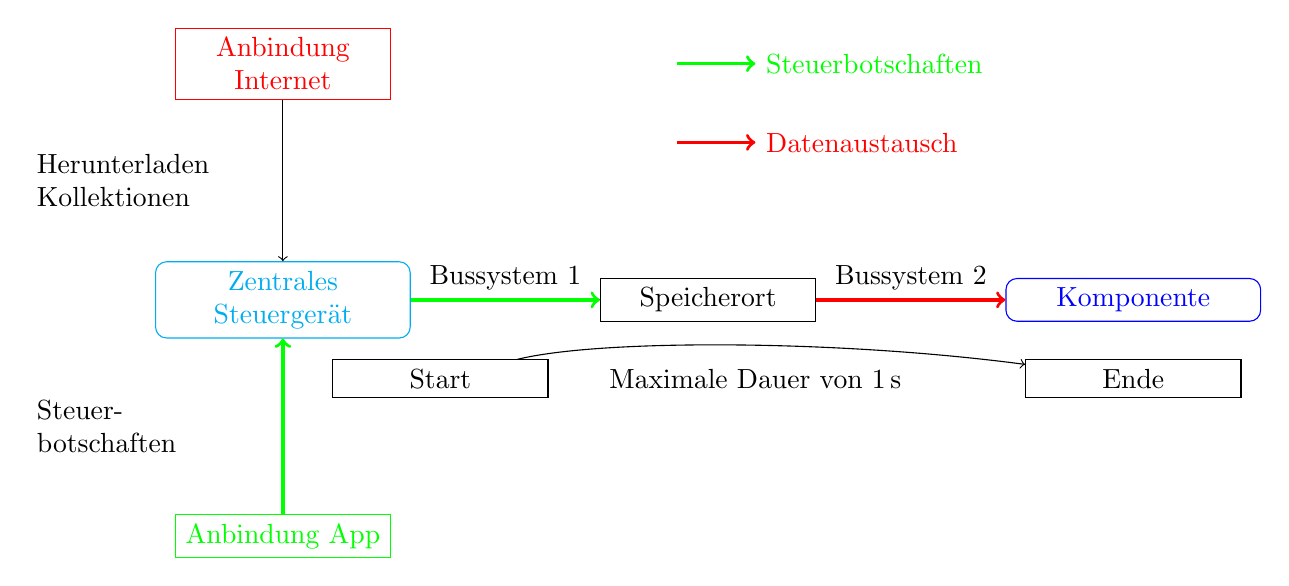
\begin{tikzpicture}[first/.style={draw, text width=3cm, align=center, rounded corners}, second/.style={draw, text width=2.5cm, align=center}]
	\node[first, cyan] (Z) at (0,0) {Zentrales Steuergerät};
	\node[second, red] (C) at (0,3) {Anbindung Internet};
	\node[second, green] (D) at (0,-3) {Anbindung App};
	\node[first, blue] (K1) at (10.8,0) {Komponente};
	\node[second] (S1) at (5.4,0) {Speicherort};
	\draw[<-] (Z) -- node[left,text width=3cm] {Herunterladen Kollektionen} (C);
	\draw[] (Z) -- node[left,text width=3cm] {Steuer-\\botschaften} (D);
	\draw[] (Z) -- node[above] {Bussystem 1} (S1);
	\draw[] (S1) -- node[above] {Bussystem 2} (K1.west);
	\draw[->, green, very thick] (D) -- (Z);
	\draw[->, green, very thick] (Z) -- (S1);
	\draw[->, red, very thick] (S1) -- (K1);
	\draw[->, green, very thick] (5, 3) -- (6,3) node[right] {Steuerbotschaften};
	\draw[->, red, very thick] (5, 2) -- (6, 2) node[right] {Datenaustausch};
	\node[second] (S) at (2, -1) {Start};
	\node[second] (E) at (10.8, -1) {Ende};
	\draw[->] (S) .. controls (4, -0.5) and (7, -0.5) .. (E);
	\node (B) at (6,-1) {Maximale Dauer von $ 1\,\mathrm{s} $};
\end{tikzpicture}
	\caption[Anforderung 1: Umschalten zwischen Kollektionen in unter einer Sekunde]{Anforderung 1: Umschalten zwischen Kollektionen in unter einer Sekunde}
	\label{fig:anforderung1}
\end{figure}
\begin{figure}[hbt]
	\centering
	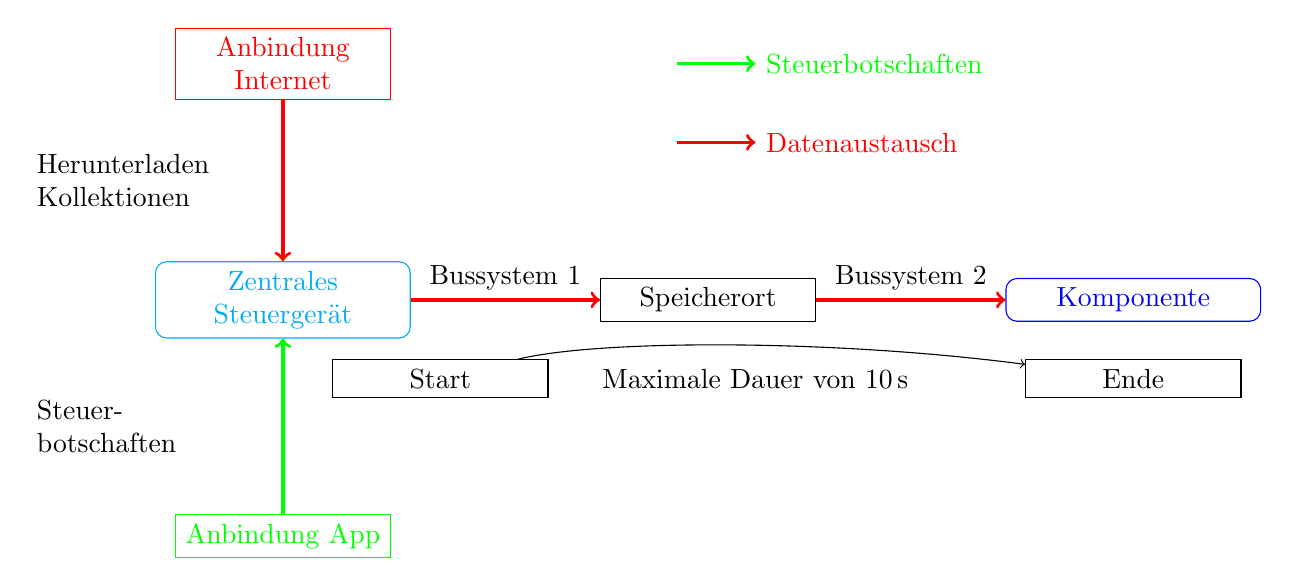
\begin{tikzpicture}[first/.style={draw, text width=3cm, align=center, rounded corners}, second/.style={draw, text width=2.5cm, align=center}]
	\node[first, cyan] (Z) at (0,0) {Zentrales Steuergerät};
	\node[second, red] (C) at (0,3) {Anbindung Internet};
	\node[second, green] (D) at (0,-3) {Anbindung App};
	\node[first, blue] (K1) at (10.8,0) {Komponente};
	\node[second] (S1) at (5.4,0) {Speicherort};
	\draw[-] (Z) -- node[left,text width=3cm] {Herunterladen Kollektionen} (C);
	\draw[-] (Z) -- node[left,text width=3cm] {Steuer-\\botschaften} (D);
	\draw[-] (Z) -- node[above] {Bussystem 1} (S1);
	\draw[-] (S1) -- node[above] {Bussystem 2} (K1.west);
	\draw[->, green, very thick] (5, 3) -- (6,3) node[right] {Steuerbotschaften};
	\draw[->, red, very thick] (5, 2) -- (6, 2) node[right] {Datenaustausch};
	\draw[->, green, very thick] (D) -- (Z);
	\draw[->, red, very thick] (C) -- (Z);
	\draw[->, red, very thick] (Z) -- (S1);
	\draw[->, red, very thick] (S1) -- (K1);
	\node[second] (S) at (2, -1) {Start};
	\node[second] (E) at (10.8, -1) {Ende};
	\draw[->] (S) .. controls (4, -0.5) and (7, -0.5) .. (E);
	\node (B) at (6,-1) {Maximale Dauer von $ 10\,\mathrm{s} $};
\end{tikzpicture}
	\caption[Anforderung 2: Anzeigen einer neuen Kollektion in unter zehn Sekunde]{Anforderung 2: Anzeigen einer neuen Kollektion in unter zehn Sekunde}
	\label{fig:anforderung2}
\end{figure}
\section{Implementierungsoptionen}
Jede Komponente besteht aus einer Anzeigefläche mit einer dazugehörigen Steuerung, die aus Bild oder Videodateien die einzelnen Bildpunkte setzt. Diese Komponente kann sich überall im Fahrzeug befinden.
Das Fahrzeug verfügt über ein zentrales Steuergerät, dass neue Kollektion aus dem Internet herunterladen kann und die Bedienbefehle der App erhält.
\paragraph{Speicherort}
Der Speicherort der Daten kann an unterschiedlichen Stellen im Fahrzeug liegen. Entweder die Daten sind gesammelt in dem zentralen Steuergerät gespeichert oder die Daten sind direkt bei den Komponenten gespeichert. Eine dritte Option ist die Bündelung der Daten von Komponenten, die sich in der Nähe befinden.
Nachfolgend werden die drei mögliche Varianten in den Diagrammen \ref{fig:architektur1}, \ref{fig:architektur2}  und \ref{fig:architektur3} skizziert.
\begin{figure}[hbt]
	\centering
	
\begin{tikzpicture}
	\node[text width=3.2cm, align=center] (Computer) {Computer};
\end{tikzpicture}
	\caption[Positionierung Dateispeicher im zentralen Steuergerät]{Positionierung Dateispeicher im zentralen Steuergerät}
	\label{fig:architektur1}
\end{figure}
\begin{figure}[hbt]
	\centering
	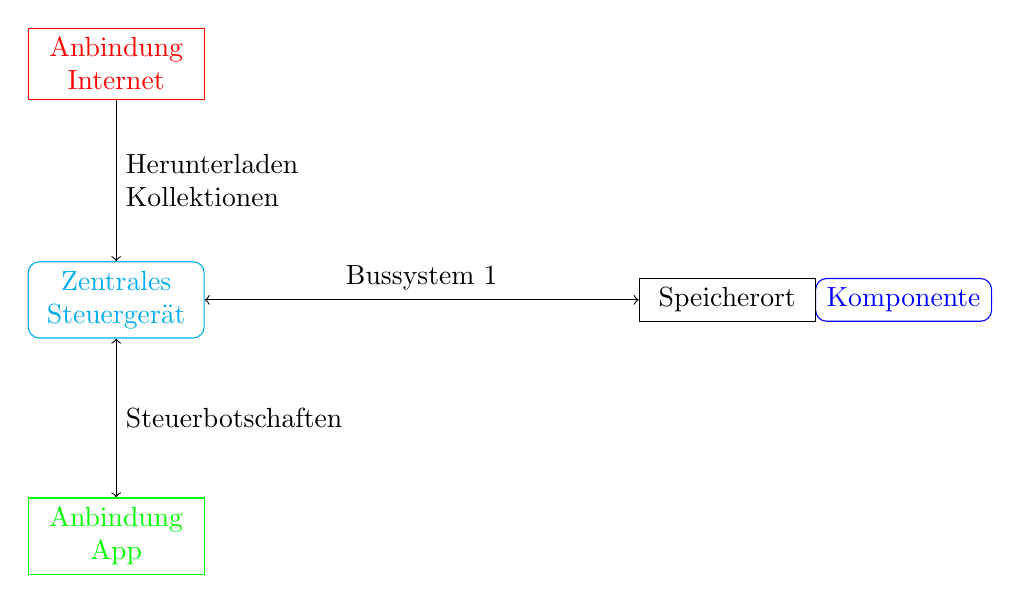
\begin{tikzpicture}[first/.style={draw, text width=2cm, align=center, rounded corners}, second/.style={draw, text width=2cm, align=center}]
	\node[first, cyan] (Z) at (0,0) {Zentrales Steuergerät};
	\node[second, red] (C) at (0,3) {Anbindung Internet};
	\node[second, green] (D) at (0,-3) {Anbindung App};
	\node[first, blue] (K) at (10,0) {Komponente};
	\node[second] (S) at (7.76,0) {Speicherort};
	\draw[<-] (Z) -- node[right,text width=2.5cm] {Herunterladen Kollektionen} (C);
	\draw[<->] (Z) -- node[right,text width=2.5cm] {Steuerbotschaften} (D);
	\draw[<->] (Z) -- node[above] {Bussystem 1} (S);
	%\draw[<->] (S) -- node[above] {Bussystem 2} (K);
\end{tikzpicture}
	\caption[Positionierung Dateispeicher lokal an der Komponente]{Positionierung Dateispeicher lokal an der Komponente}
	\label{fig:architektur2}
\end{figure}
\begin{figure}[hbt]
	\centering
	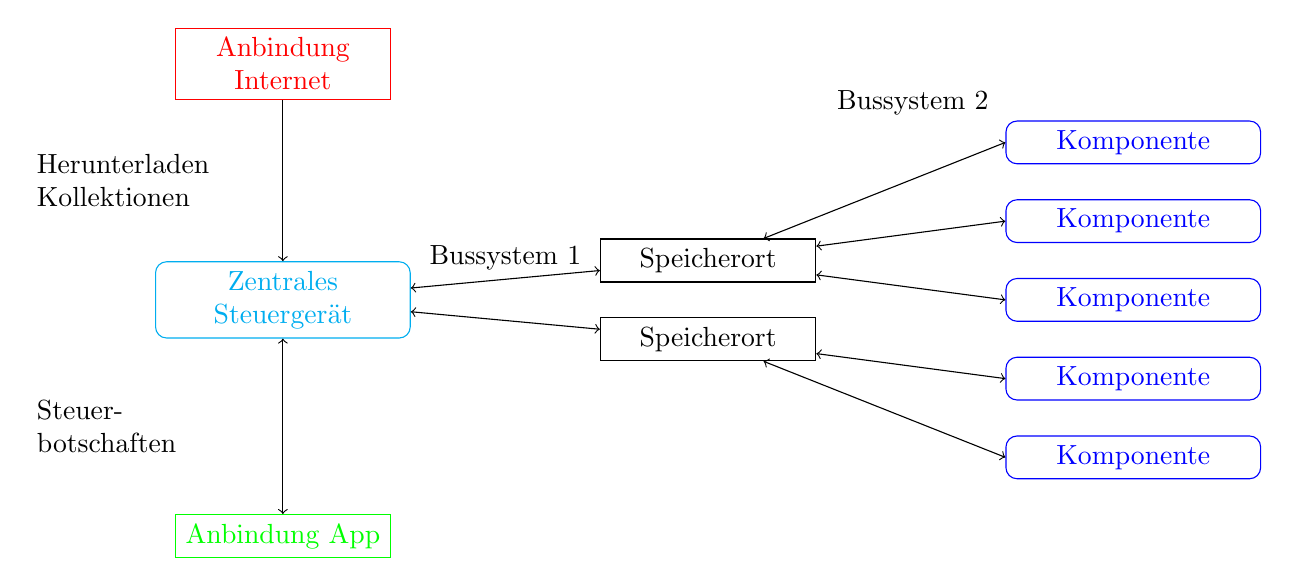
\begin{tikzpicture}[first/.style={draw, text width=3cm, align=center, rounded corners}, second/.style={draw, text width=2.5cm, align=center}]
	\node[first, cyan] (Z) at (0,0) {Zentrales Steuergerät};
	\node[second, red] (C) at (0,3) {Anbindung Internet};
	\node[second, green] (D) at (0,-3) {Anbindung App};
	\node[first, blue] (K1) at (10.8,2) {Komponente};
	\node[first, blue] (K2) at (10.8,1) {Komponente};
	\node[first, blue] (K3) at (10.8,0) {Komponente};
	\node[first, blue] (K4) at (10.8,-1) {Komponente};
	\node[first, blue] (K5) at (10.8,-2) {Komponente};
	\node[second] (S1) at (5.4,0.5) {Speicherort};
	\node[second] (S2) at (5.4,-0.5) {Speicherort};
	\draw[<-] (Z) -- node[left,text width=3cm] {Herunterladen Kollektionen} (C);
	\draw[<->] (Z) -- node[left,text width=3cm] {Steuer-\\botschaften} (D);
	\draw[<->] (Z) -- node[above] {Bussystem 1} (S1);
	\draw[<->] (Z) -- (S2);
	\node at (8, 2.5) {Bussystem 2};
 	\draw[<->] (S1) -- (K1.west);
	\draw[<->] (S1) -- (K2.west);
	\draw[<->] (S1) -- (K3.west);
	\draw[<->] (S2) -- (K4.west);
	\draw[<->] (S2) -- (K5.west);
\end{tikzpicture}
	\caption[Positionierung Dateispeicher zwischen zentralen Steuergerät und Komponente]{Positionierung Dateispeicher zwischen zentralen Steuergerät und Komponente}
	\label{fig:architektur3}
\end{figure}
Abhängig vom Speicherort müssen die Bussysteme eine genügend hohe Bandbreite besitzen, um die Anforderungen einzuhalten. 

\section{Vergleich der unterschiedlichen Lösungsansätze}